
\chapter{Background}

\begin{chapquote}{\textit{Arthur C. Clarke}}
    ``Before you become too entranced with gorgeous gadgets and mesmerizing video displays, let me remind you that information is not knowledge, knowledge is not wisdom, and wisdom is not foresight. Each grows out of the other, and we need them all''
\end{chapquote}

\section{Geometry in Computer Vision}

The pixel is the building block of digital imagery. Thanks to our ability to fabricate advanced circuits on the scale of nanometers, digital camera sensors have become ubiquitous - making their way into all manner of consumer devices. Because the photodiodes in camera sensors are typically arranged on a 2D plane, most of our operations on digital images manipulate the 2D structures present in that pixel data. However, it is important to remember that the 2D shapes and structures that appear on the sensor plane are projected versions of a 3D world. 

\subsection{The Pinhole Camera}

The most basic kind of camera, the pinhole camera projects a 3D world point $[X, Y, Z]$ to a homogenous coordinate on a 2D plane $[u, v, w]$. This relationship is captured in the $3 \times 3$ camera intrinsics matrix and is typically written as 

\begin{equation}
\begin{bmatrix}
    u\\
    v\\
    w
\end{bmatrix} = 
\begin{bmatrix}
    f_x & s & u_0 \\ 
    0 & f_y  & v_0 \\ 
    0 & 0 & 1 
\end{bmatrix}
\begin{bmatrix}
    X \\
    Y \\
    Z
\end{bmatrix}.
\end{equation}

The intrinsics matrix can alternatively be thought of as mapping ray directions to pixel coordinates:

\begin{equation}
\begin{bmatrix}
    u\\
    v\\
    1
\end{bmatrix} = 
\begin{bmatrix}
    f_x & s & u_0 \\ 
    0 & f_y  & v_0 \\ 
    0 & 0 & 1 
\end{bmatrix}
\begin{bmatrix}
    tan(\theta) \\
    tan(\phi) \\
    1
\end{bmatrix}.
\end{equation}


\begin{figure}[htbp]
    \centering 
    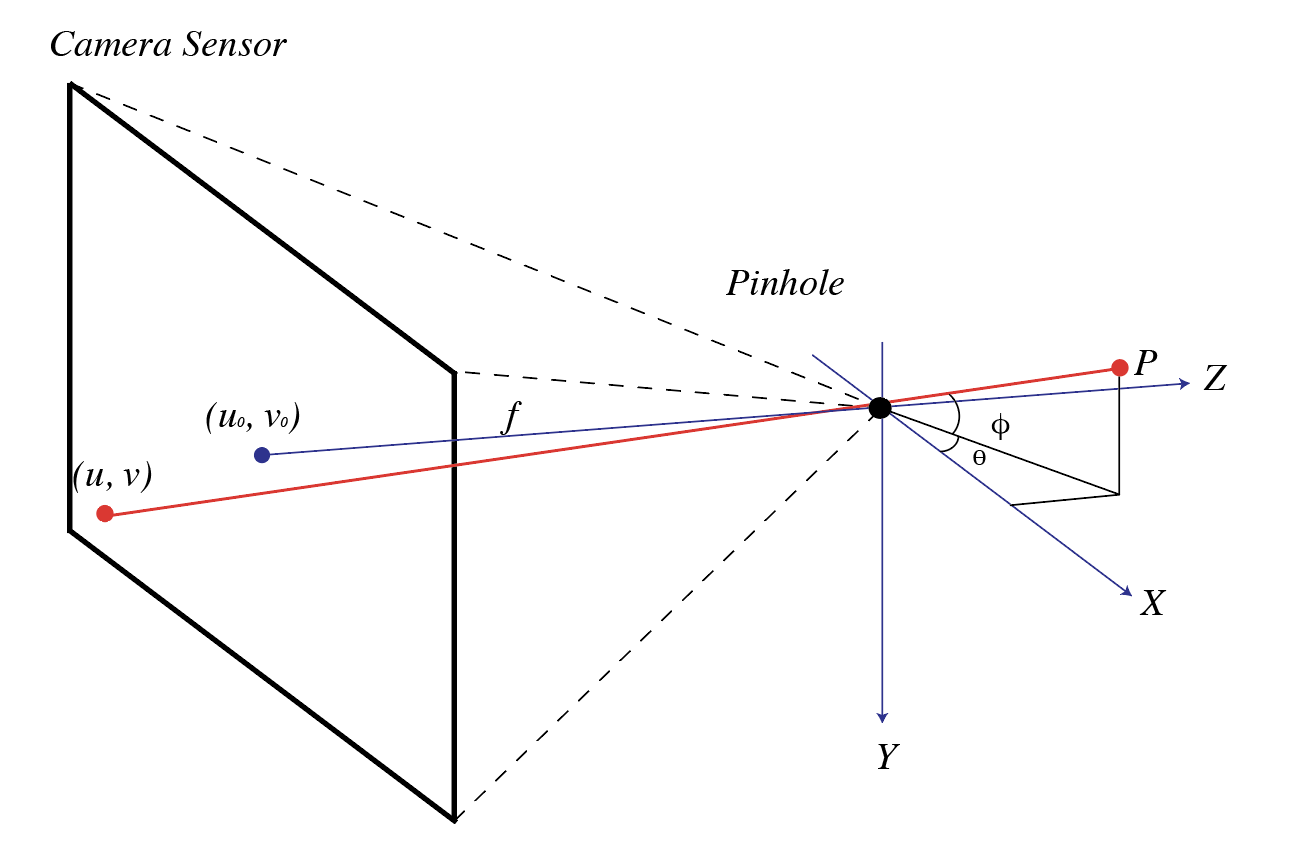
\includegraphics[width=4in]{images/pinhole.png}
    \caption[The pinhole model of the camera]{The pinhole model describes how a light ray originating from world coordinate $P$ is received at pixel coordinate $(u, v)$. Equivalently, the pinhole model can be thought of as associating the light ray of elevation $\phi$ and azimuth $\theta$ with the specific pixel coordinate $(u, v)$. Since the relationship is a one-to-one mapping between ray directions and pixel coordinates, the inverse of the intrinsics matrix $K^{-1}$ associates each pixel with a corresponding ray direction.}
\end{figure}



\subsection{Epipolar Geometry and the Fundamental Matrix}

Epipolar geometry describes the relationship between two cameras, and imposes a set of constraints which makes it possible for us to draw meaningful geometric information when we have two views of the same scene. This relationship is encapsulated in a $3 \times 3$ matrix called the Fundamental matrix $F$. The culmination of the epipolar constraint is that any point in 3 dimensional space that appears at pixel $(u_1, v_1, 1)$ in one view and $(u_2, v_2, 1)$ in the second view must satisfy the relationship:

\begin{equation}
    \begin{bmatrix}
        u_1, v_1, 1
    \end{bmatrix}^T
    F
    \begin{bmatrix}
        u_2, v_2, 1
    \end{bmatrix}
    = 0.
\end{equation}

\begin{figure}
    \centering
    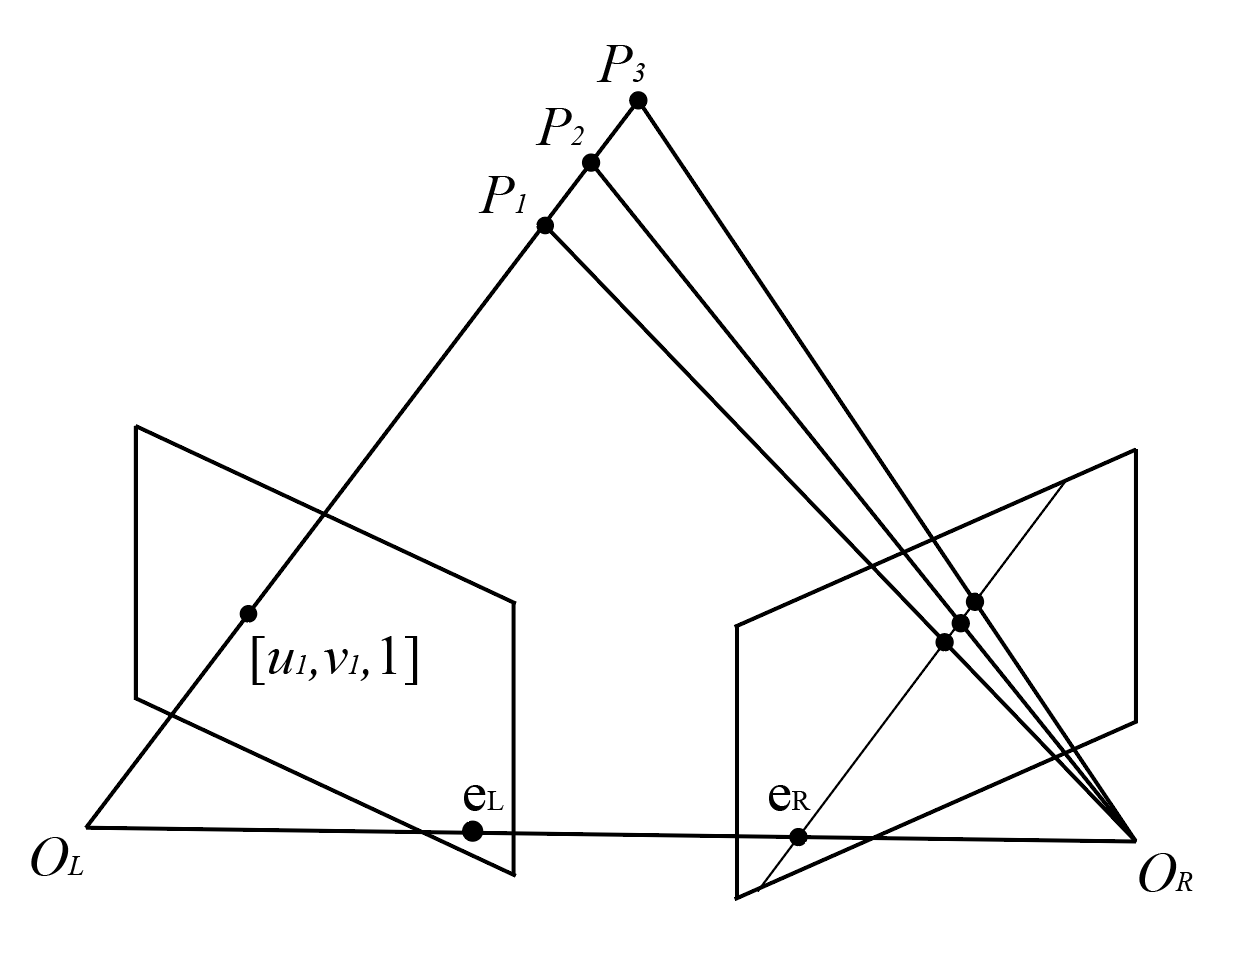
\includegraphics[width=2.5in]{images/epipolarplane.png}
    \caption[The fundamental matrix in epipolar geometry]{Epipolar geometry is the geometry of stereo camera pairs. Without knowing depth, the point $[u,v,1]$ can be projected to any number of points $P1, P2, P3... $ in 3D space, having many possible projections on the sensor plane of the right camera. The Fundamental matrix however constrains the set of possible projections to lie on a straight line called the epipolar line.}
    \label{epipolarplane}
\end{figure}

The Fundamental matrix thus describes the rotation and translation between two cameras up to scale. Any point projected from pixel coordinate $[u_1, v_1, 1]$ must lie on the epipolar line in the second image, which is formed by the intersection of the epipolar plane and the imaging plane. 



\section{The 4D Light Field}
Light field imaging has emerged as a powerful tool in computer vision for robotics, offering a rich higher-dimensional representation than what can be captured by conventional optics. The underlying principle used to describe the light field is the plenoptic function, a 7-dimensional mapping that assigns radiance values to the light rays at every position in space, in every orientation, at all wavelengths, throughout all of time \cite{adelson1991plenoptic}. This can be formally expressed as $L(x,y,z,\theta, \phi, \lambda, t)$, and measured in $W/m^2/sr/nm/s$. 


Levoy et al. \cite{levoy1996lfrendering} shows that with the addition of practical constraints however, the plenoptic function can be expressed more concisely as a parameterisation of 4 variables. Pixels on camera sensors integrate the number of photons arriving at them over a finite period of time removing the temporal dimension, and each colour channel can be thought of as a monochromatic sampling of the light field, removing the spectral dimension. Additionally, and importantly, is the constraint that the radiance of light rays propagating through a vacuum do not change if samples are restricted to the convex hull of the scene, thus reducing the overall dimensionality of the plenoptic function by one additional parameter \cite{levoy1996lfrendering}. To illustrate this, one could think of the light rays leaving the inside of a bowl sat upright on a table. Many of those rays may only travel a small distance before being blocked by the inside of the bowl itself, meaning those rays will never be registered by any practical measurement device. As shown in Figure 2.3 if we consider only the convex hull of the bowl however, we are required only to represent the value of the plenoptic function on the encapsulating surface of the object \cite{gortler1996lumigraph}.

\begin{figure}[htbp]
    \centering
    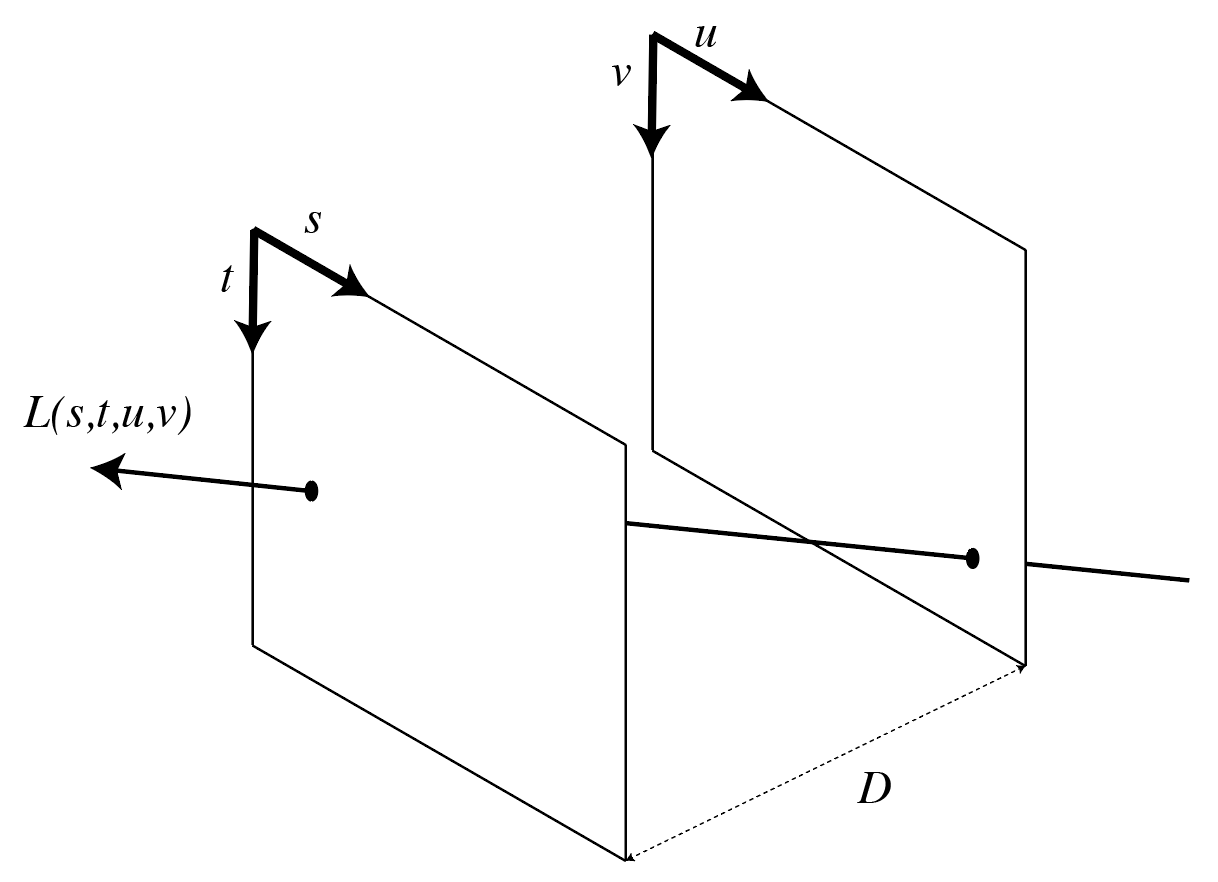
\includegraphics[width=2.5in]{images/2pp.png}
    \label{convexhull}
    
\includegraphics[width=0.3in]{images/blank.png}
    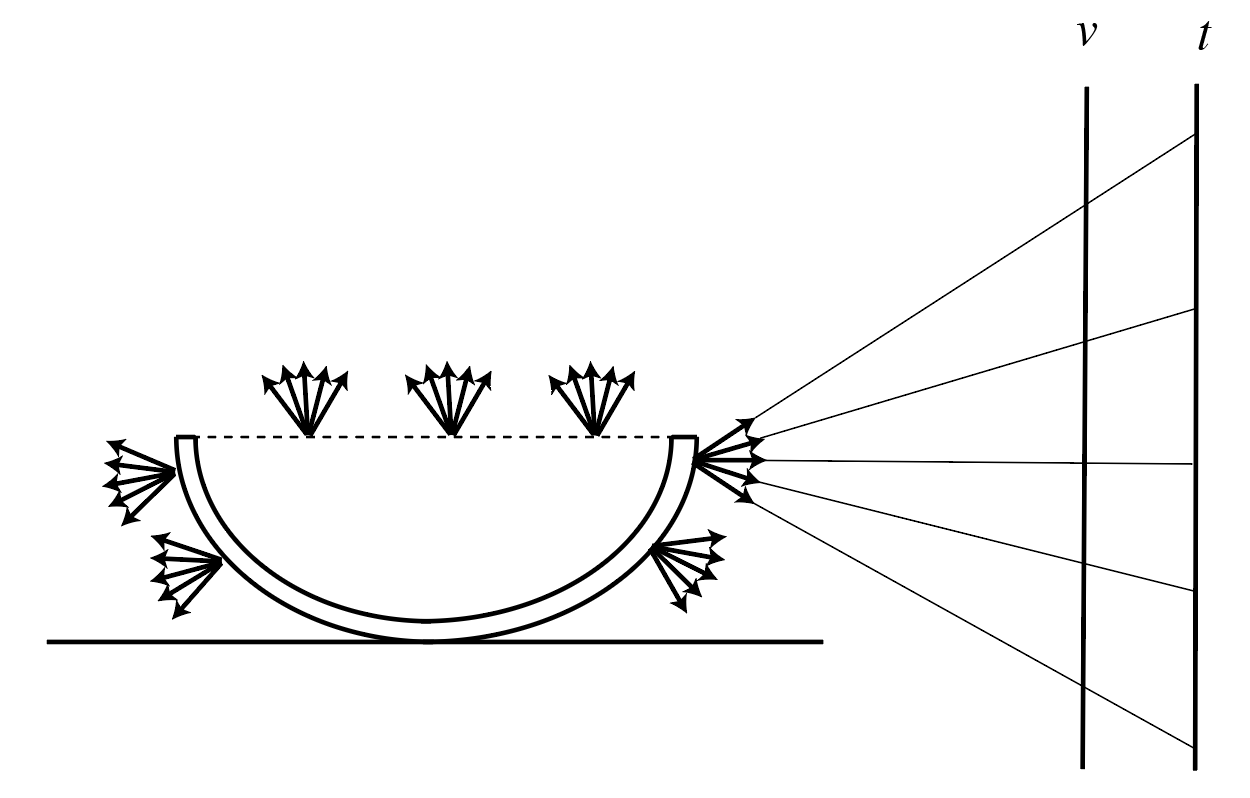
\includegraphics[width=2.5in]{images/convexhull.png}
    
    \caption[The two-plane parameterisation and the free-space assumption]{Two-plane parameterisation (left): the plenoptic function can be described by the radiance along a ray passing through two parallel planes. The free space assumption (right): if we consider only the bundle of rays leaving from the convex hull of the object at a particular instance in time, in a single colour channel, we can parameterise the light rays as a function of 4 variables rather than 7.}
    
    
\end{figure}

Also illustrated is a common convention for describing light rays in this 4 dimensional space called the two plane parameterisation \cite{gortler1996lumigraph}. In this parameterisation, two parallel planes are used to fix both the position and orientation of each ray by fixing their points of intersection with two parallel planes. By convention, the plane closest to the scene is termed \textit{u, v} and the plane closest to the camera sensor is the \textit{s, t} plane.

This 4D realisation of the light field originated as a model of rendering 3D computer graphics, one which shifted emphasis from notions of texture and geometric primitives to modeling the behaviour of light rays permeating space. Since then however, the conceptual framework of the light field has drawn a following of researchers at an intersecting region of signal processing, computer vision and robotics \cite{dansereau2014phd}. This notion of light field imaging finds a foothold in this work through the utilisation of camera arrays, which are devices that sample multiple views of the same scene. Using a camera array is a simple method for acquiring a sparse sample of the light field, where the position of the camera determines \textit{(s,t)} while the location of the pixel determines \textit{(u, v)} \cite{yao2016camarray}. The images captured from a camera array are mapped easily to the 4D light field, and identifying corresponding pixels across images exposes a rich tapestry of geometric information about the scene. 


\begin{figure}[tbp]
    \centering
    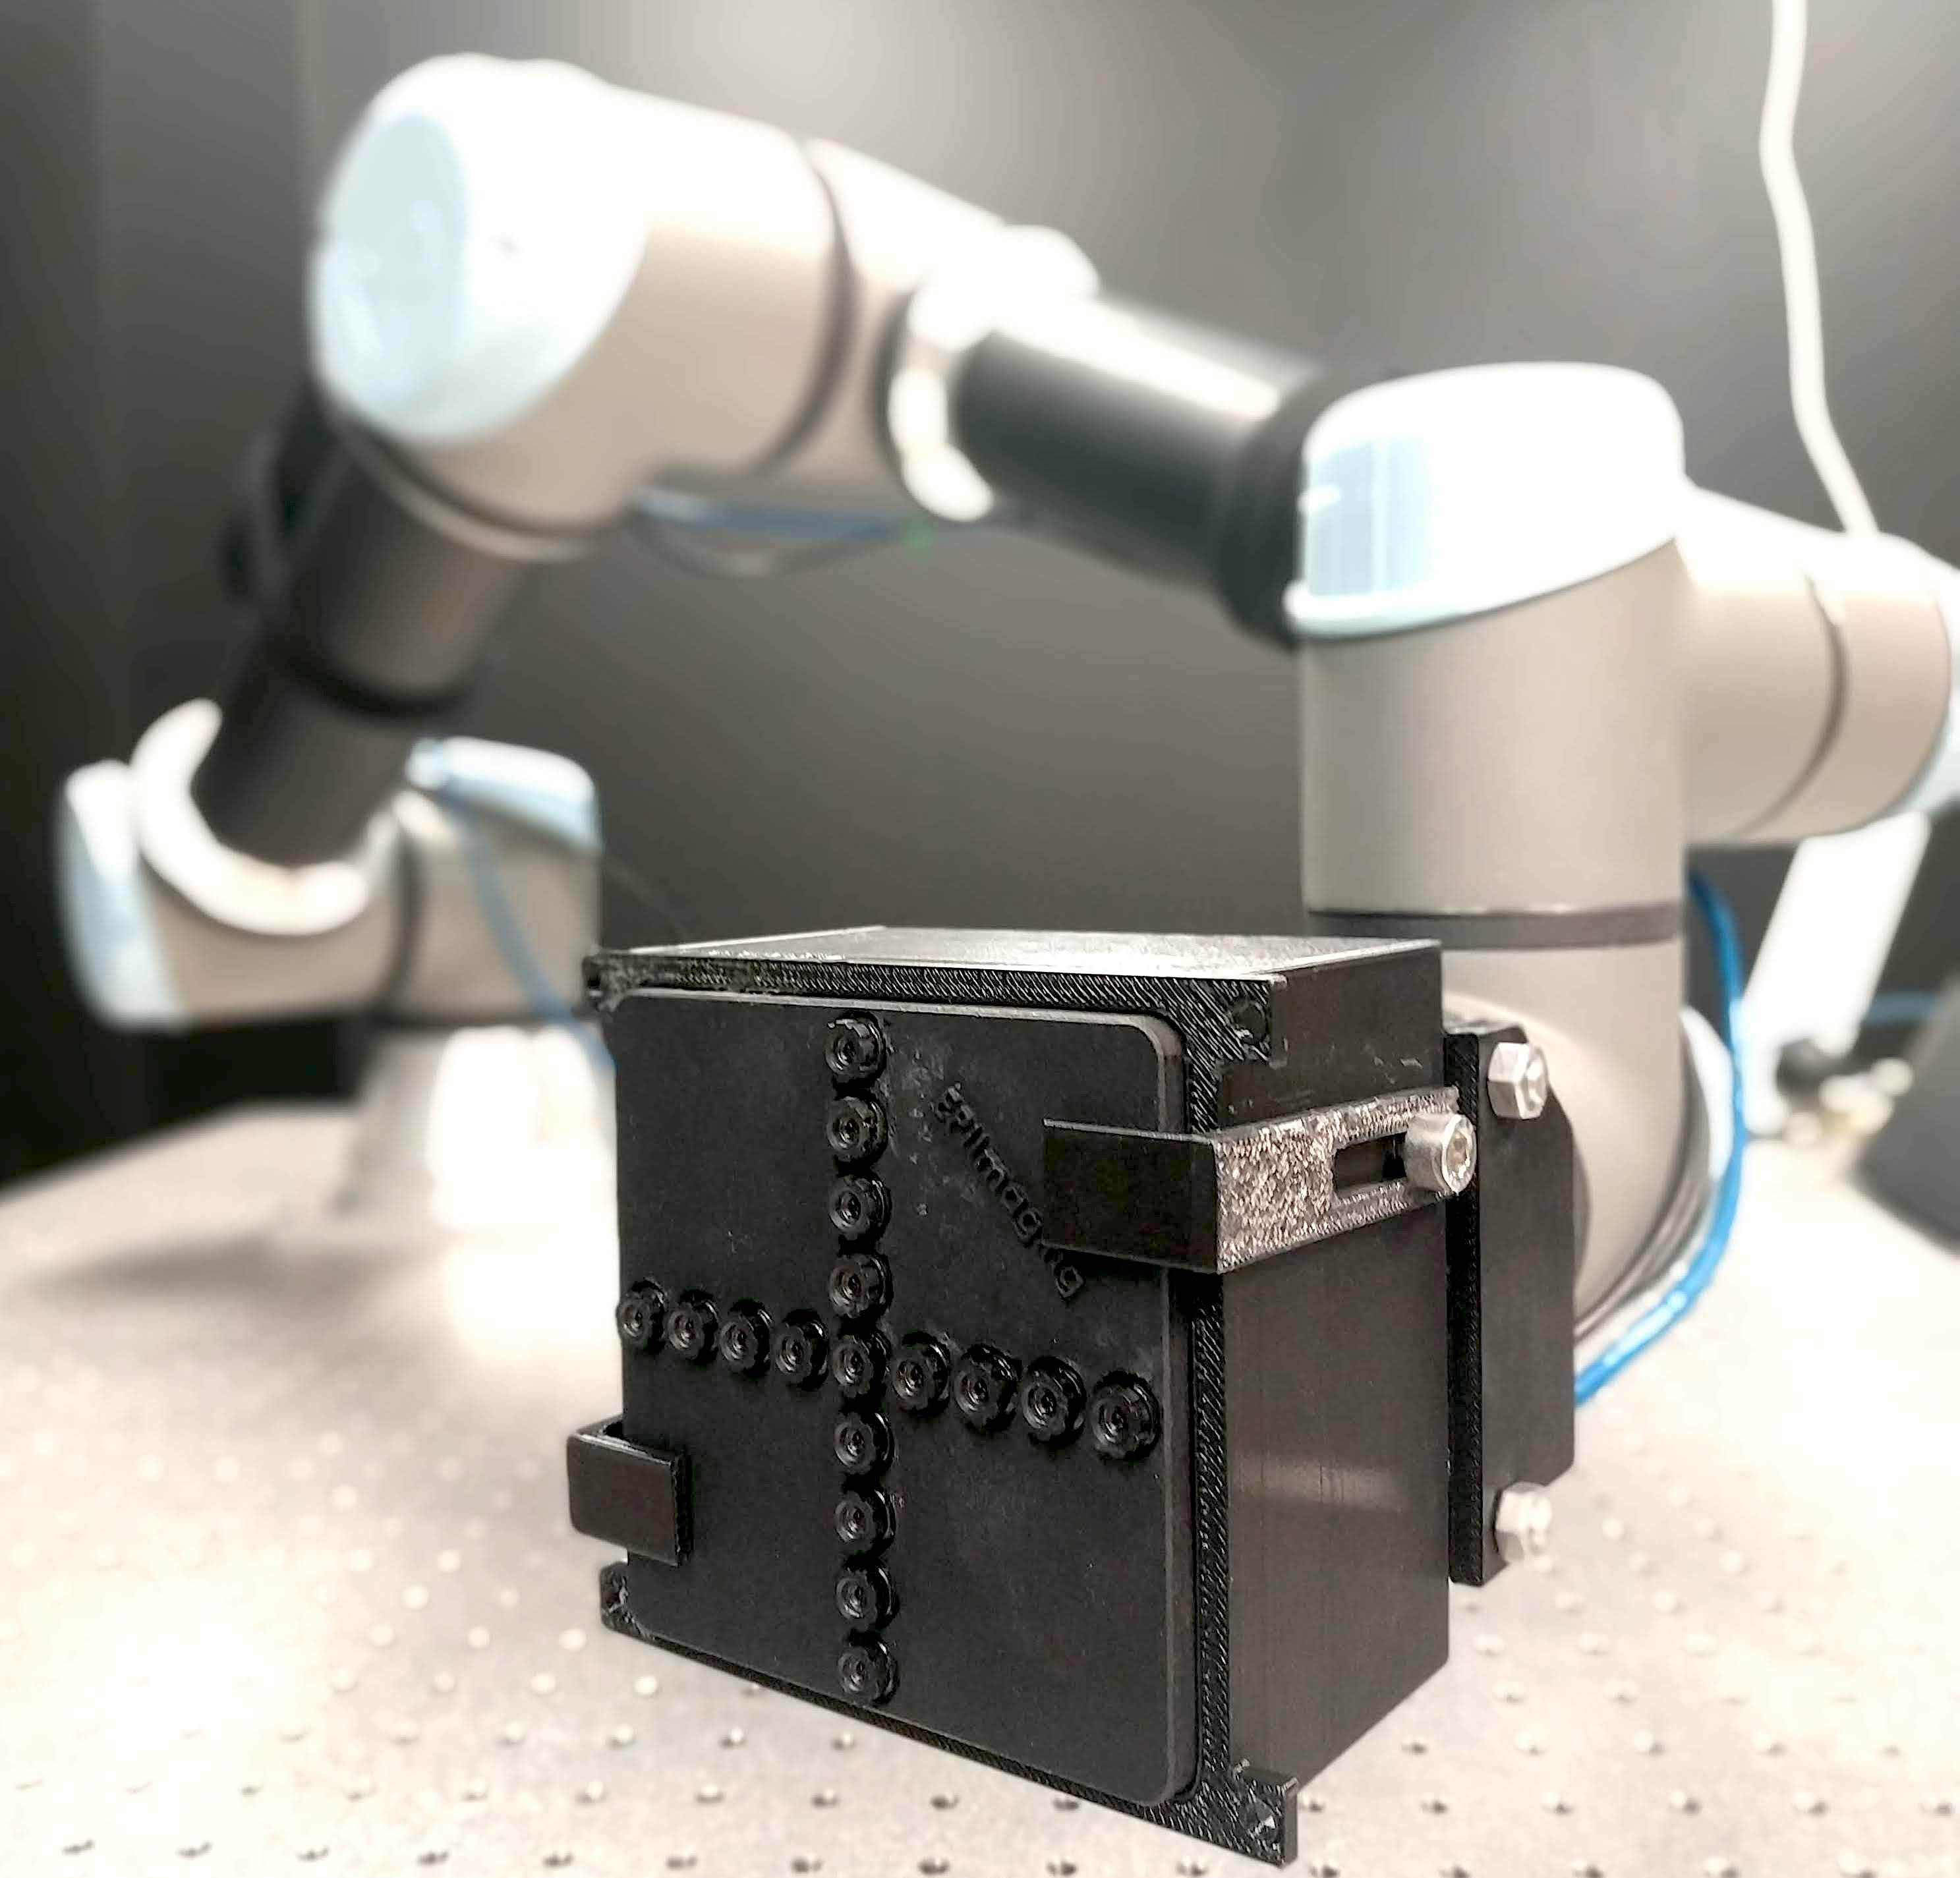
\includegraphics[width=4.5in]{images/robotcamera.jpg}
    \caption{An example of a camera array mounted on a robotic arm. This camera array is configured as 17 sub-apertures arranged on a single plane in a cross-hair formation. Camera arrays sample several views of the same scene and are thus capable of acquiring a sparse sample of the light field. This is the camera that will be used throughout this thesis project.}
    \label{cameraarray}
    \vspace{1cm}
    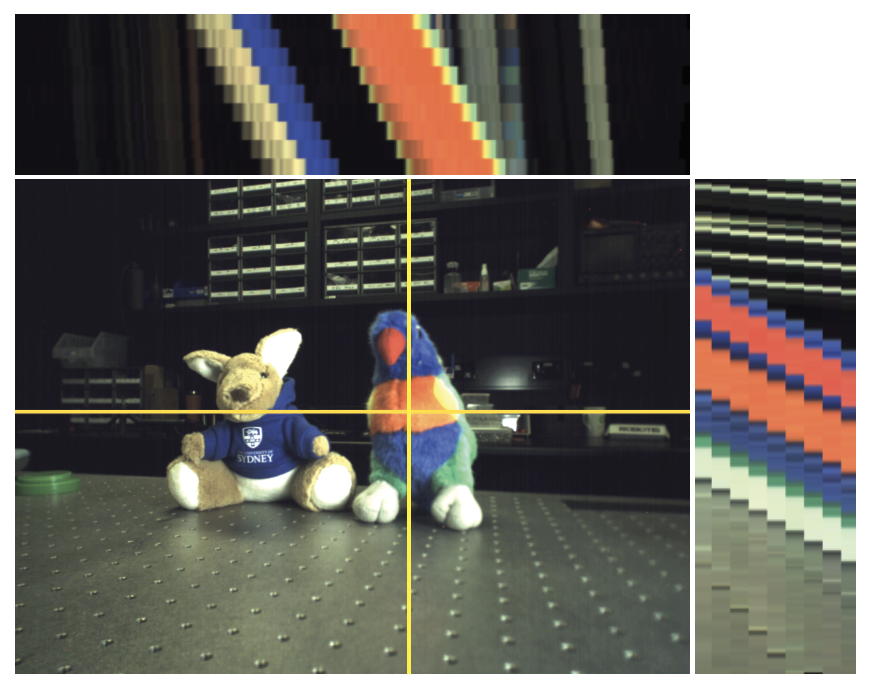
\includegraphics[width=2in]{images/epipolarimage.png}
    
\includegraphics[width=0.4in]{images/blank.png}
    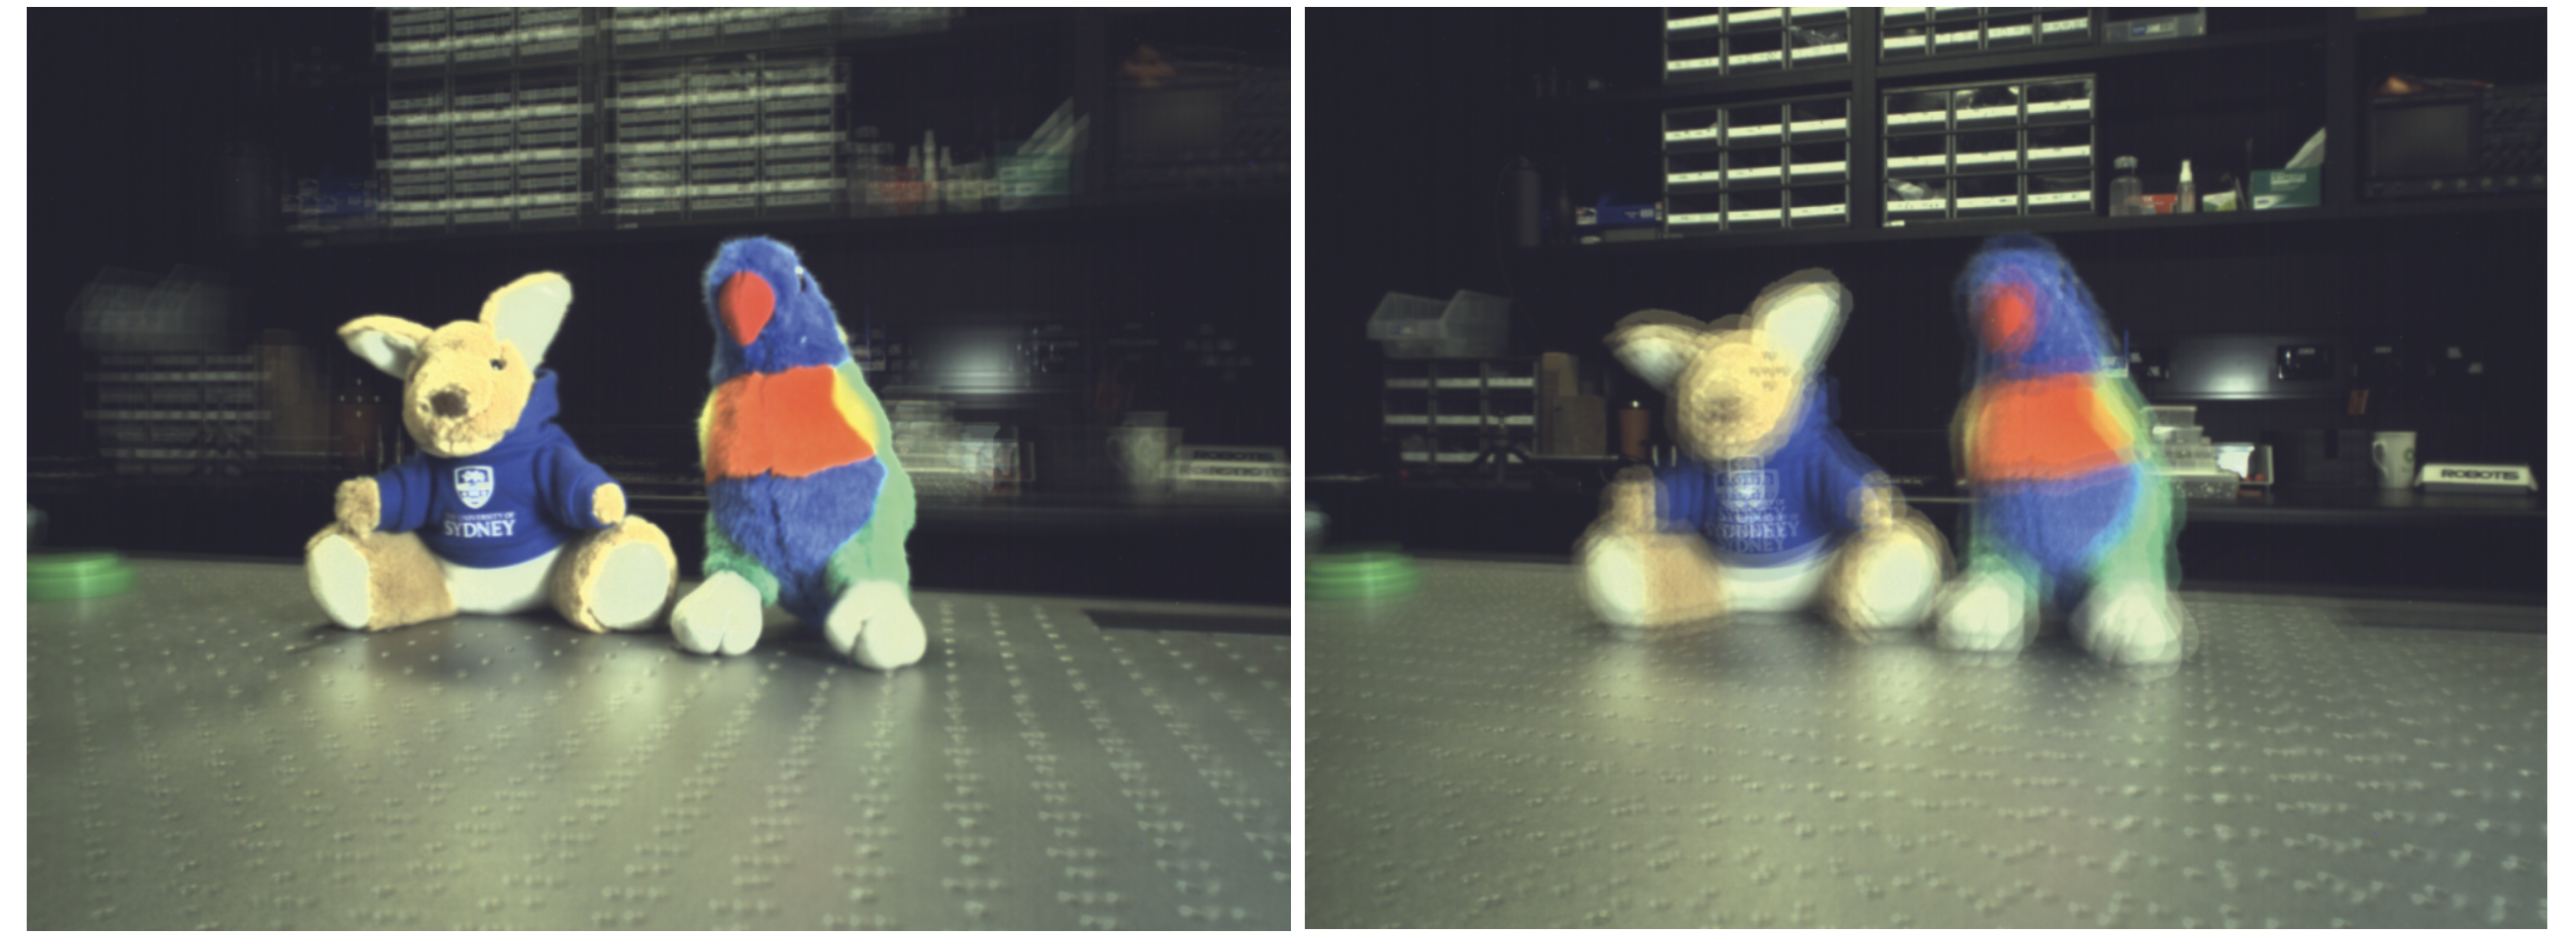
\includegraphics[width=3.5in]{images/refocus.png}
    \caption{Epipolar Plane Images (left): Shown as a slice of a volume, the images formed by dissecting the image in the \textit{s,u} and \textit{t,v} planes are characterised by sheared straight lines, with the grade of the slope encoding the amount of parallax experienced by a pixel at that \textit{u} or \textit{v} coordinate. Synthetic aperture focusing (right): taking the average of every image from the camera array yields an image where different parts are in focus depending on the alignments of the images.}
    \label{epiplaneimg}
\end{figure}


One way that this geometric information can be easily visualised is by taking slices of the light field image in the \textit{s,u} or \textit{t, v} axes as shown in Figure \ref{epiplaneimg}. While the idea of taking a 2D slice from the 4D image can seem complex, the task of generating a so called `epipolar plane image' from a camera array is deceptively simple. Images captured from camera arrays can be stacked to form a solid volume, from which 2D slices can be sampled. Each of these slices yields an image characterised by sheared straight lines, encoding information about the geometry of the scene, including depth and occlusions \cite{bolles1987epiplane}. 

The geometric information encoded in a light field sampling can alternatively be visualised by processing the image into a `focal stack'. Focal stacks closely resemble images with shallow depth of field such as those that can be captured from a commercial DSLR camera. Light field focal stacks differ from focus in the optical sense however in that they are synthetic and can be recomputed after the image has been taken, effectively allowing control over the depth of field and focal depth in post-processing. Focal stacks can be computed from camera array images by layering images over one another and taking the average value for each pixel. The result is that parts of the scene that closely overlap appear in focus while areas with poor overlap create a `bokeh' effect. More formally, if the relative pose of each camera is known, a specific focal stack for any desired depth can be computed by projecting each image onto the desired focal plane, and computing their average \cite{vaish2004parallax}.

These representations of the light field play an important role in this thesis project as we experiment with different methods for feeding light field images to the machine learning pipeline. An important consideration in any machine learning algorithm is the feature space - based on what particular inputs will the algorithm be making its decision? Raw images contain millions of measurements and thus represent an incredibly high-dimensional feature space for neural networks to process. Light field images are several times larger, and thus it is important that some form of dimensionality reduction is used to ease the training process. With the goal of investigating effective methods of feeding light fields to neural networks, this thesis will explore the use of three different light field formats as the entry point to the machine learning pipeline. The first two will be the focal stack, and epipolar plane image described above, interpreting the images as a 3 dimensional volume created by stacking 2 dimensional images on top of one another. The third will treat the light field as a 4 dimensional volume, requiring a 4D signal processing pipeline to fully take advantage of the dimensionality.

\section{Machine Learning in Computer Vision}


An oft-quoted anecdote in computer vision tells of MIT researcher Seymour Papert, who in 1966 assigned a summer project that sounded simple enough, namely to construct a `visual system' that could describe what objects it saw by name \cite{papert1966vision}. While the regimes of computer vision have evolved substantially since 1966, many of the ideas, and challenges have persisted. This is embodied in the popularity of projects such as the ImageNet Large Scale Visual Recognition Challenge (ILSVRC) \cite{ilsvrc}, drawing researchers from institutions around the world. It was at the ILSVRC annual challenge where in 2012, a convolutional neural network achieved a top-5 error rate of 15.3\%, outperforming all previous submissions by 10.8\% \cite{krizhevsky2012alexnet}. Until `AlexNet' in 2012, the competition consisted of competitors introducing algorithms that produced marginal improvements year on year. Needless to say, an improvement of over 10\% generated noise in the computer vision community, drawing attention to the powerful capabilities of deep learning.

While deep neural networks for computer vision have gained massive popularity since the success of AlexNet, the history of neural architecture models begins much earlier, with the perceptron as described by Frank Rosenblatt in \cite{rosenblatt1959neurodynamics}. The fundamental building block of neural networks, the `perceptron' is a module that accepts several inputs, and produces a single output computed as a weighted sum of each input - allowing complex functions to be approximated when several perceptrons are layered together as a `multilayer perceptron' \cite{minsky1969perceptrons}. The process of finding the optimal set of weights that produce the desired output given a set of inputs is referred to as training, and in practice is usually found by optimising some cost function using the backpropagation algorithm \cite{rumelhart1986backprop}. Backpropagation uses the chain rule of calculus to calculate partial derivatives of each weight in the network with respect to the cost function. A gradient based optimisation algorithm such as stochastic gradient descent (SGD) can then be employed to minimise the cost function. Thus, it is important that each step in the computation of a neural networks output be differentiable - that is, it must support the backpropagation of gradients or else gradient-based optimisation will fail. The `fully-differentiable' requirement for neural networks is an important consideration in this work; a novel cost function is described in Chapter 4, where each step in its computation must be differentiable with respect to the output of the previous step. 

\begin{figure}[tbp]
    \centering
    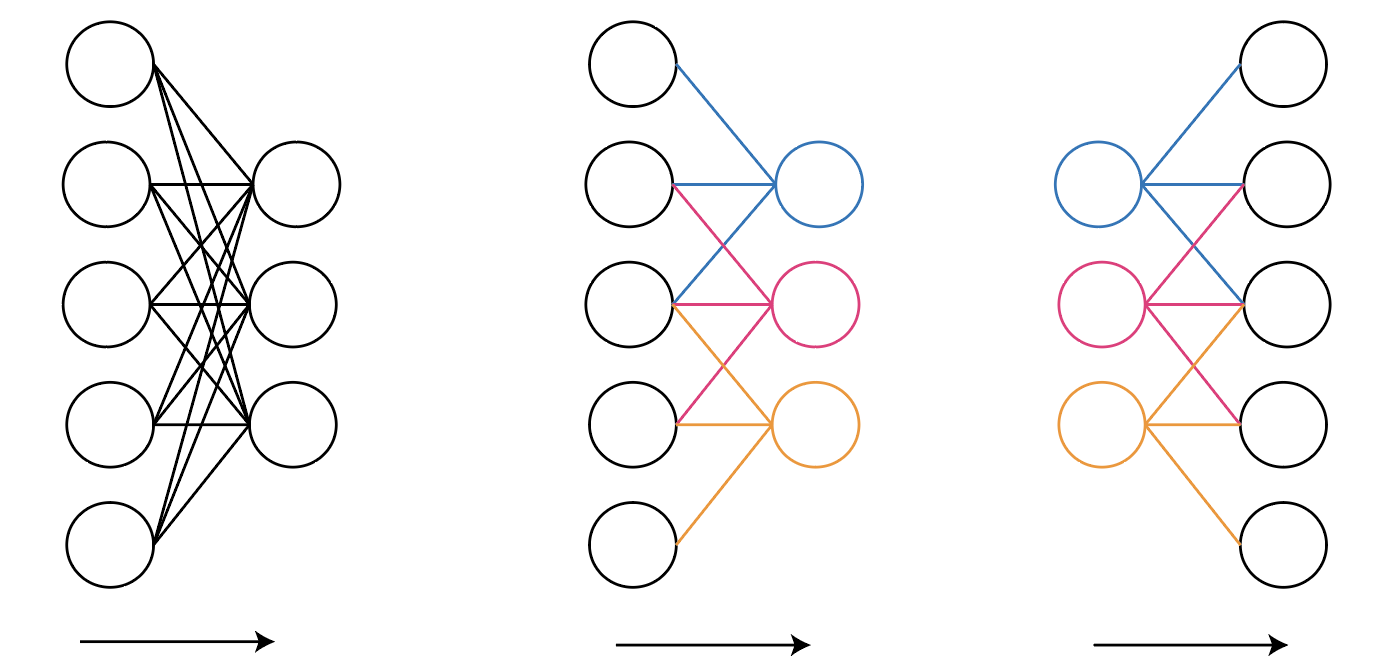
\includegraphics[width=5in]{images/cnnvsmlp.png}
    
    \caption{Multilayer Perceptron (left): each output from one layer is fed into the inputs of every node in the subsequent layer. Convolutional Neural Networks (middle) on the other hand have a `receptive field', taking advantage of the spatial coherence of pixels in image data. The convolutional upsampling operation (right) is frequently used to upsample a low-dimensional feature space, to a higher dimensional one. It is often employed as a `learned' information decompression.}
    
    \label{convexhull}
\end{figure}


Convolutional neural networks (CNN's) are similar to multilayer perceptrons, but introduce a spatial invariance that makes them particularly well suited for extracting high-level features from image data. Where multilayer perceptrons are densely connected, the connectivity pattern of each node in a CNN takes advantage of the hierarchical organisation of patterns in image data by using a `receptive field'. Biologically inspired, these nodes respond to stimuli only in their receptive field, and so they typically learn to identify salient features in the image - combinations of pixels that represent some kind of underlying structure. As these types of networks grow deeper, the features that they learn typically become more complex \cite{lecun1989cnn}. Early layers are provided with a small region of the image, typically a window between 3 and 11 pixels wide, and so will usually learn primitive features such as lines and corners. Deeper layers however may learn to combine low-level geometries, recognising higher-level features such as eyes and mouths, and eventually even human and animal faces.


CNN's are thus popular `feature extractors' in computer vision - their ability to learn to respond to different types of stimuli mean that they have been used as a dimensionality downsampling tool, taking the millions of dimensions present in digital images  and compressing them to a feature space with a much smaller number of parameters. Closely related is the convolutional upsampling operation which performs the inverse - taking a feature space and learning to upsample that feature space into something meaningful \cite{long2014fcn}. This has given rise to a particular topology of CNN called the encoder-decoder architecture, which we take advantage of to predict depth (described in detail in Chapter 4). The encoder part of a CNN is composed of a series of convolutional downsampling operations - this can be thought of as finding an efficient compression of the information stored in the image. The decoder subsequently uses this compressed form of the information to extract some meaningful information about it. One example where this architecture has been used is in \cite{long2014fcn}, which outputs a classification for each pixel in the image. In this thesis, a fully convolutional encoder-decoder architecture will be used for a similar purpose, but rather than discretely classifying each pixel, we regress their depth values (more precisely, their \textit{z}-coordinate). 